%!TeX program=pdflatex
%!TeX encoding=utf8
%!TeX spellcheck = en_US
%!TeX root = ../../messageVortex.tex

\partepigraph{No matter how hard you work, someone else is working harder.}{Elon Musk, entrepreneur}
\part{Implementation}\label{sec:implementation}
The implementation differs from the academic model in some details. It is foremost more precise than the academic model. Furthermore, it requires a strict definition of the implementation to guarantee the interoperability between different implementations.

This section focuses therefore on the details of the reference implementation. In \cref{sec:selection}, we explain the selection of algorithms used by the protocol in general. We then focus on the implementation of the transport (\cref{sec:transportImplementation}), blending (\cref{sec:blendingImplementation}), routing (\cref{sec:routingImplementation}), and accounting (\cref{sec:accountingImplementation}) layers. We then have a look at the usability (\cref{sec:usabilityImplementation}) and efficiency (\cref{sec:transportImplementation}). Aspects relevant to the implementations' usability and efficiency are covered in \cref{sec:usabilityImplementation} and \cref{sec:usabilityImplementation}.

\chapter[Selecting Algorithms, Encodings, and Protocols]{Selection of Algorithms, Encodings, and Protocols}\label{sec:selection}
In this chapter, we choose the following mandatory supported algorithms:
\begin{itemize}
	\item Encoding: ASN.1
	\item Encryption
	\begin{itemize}
		\item AES128/256
		\item Camellia128/256
	\end{itemize}
	\item Modes
	\begin{itemize}
		\item ECB
		\item GCM
	\end{itemize}
	\item Paddings
	\begin{itemize}
		\item PKCS\#1
		\item PKCS\#7
	\end{itemize}
	\item MACs
	\begin{itemize}
		\item SHA256/512
		\item RIPE-MD256
	\end{itemize}
	\item PRNG
	\begin{itemize}
		\item mrg32k3a
		\item blumMicali
	\end{itemize}
\end{itemize}

Where security-relevant, we always choose two independent algorithms. As our protocol has the means of signaling them, we may support additional algorithms without affecting communication while improving the variety of available algorithms.

In the following sections, we emphasize on the choice and the encoding used on the protocol level.

For all algorithms, we apply the following criteria:
\begin{itemize}
	\item Always focus on common standards
	\item Focus on interoperability when selecting standards
	\item Focus on efficiency (wherever possible use simple, parallelizable algorithms)
	\item When sensible and possible chose at least two unrelated algorithms (e.g., cryptographic algorithms or MACs)
\end{itemize}

\section{Encoding Scheme}
As encoding scheme, we specified ASN.1\cite{dis19878824}. It is more compact than the initially selected XML-Standard and is very common in telecommunication and encryption (e.g., the representation of X509 is in ASN.1). To maintain interoperability, we choose DER encoding as it has precisely one possible representation for every value. Such a strict definition of encoding is important when dong signing or solving puzzles in our case and is required to diagnose message paths.

On the downside, ASN-1 encoding is, unlike XML, not human readable. As we hide the messages anyway, we considered this a minor flaw, as we need to have an always extracting program to see the messages' content.

\section{Cipher Selection}
In this protocol, a lot of encryption and hashing algorithms have to be used. We should explain the choice of these algorithms. 

We decided to define fixed key sizes for symmetric ciphers as we went with block ciphers. We encode the key length in the parameters for the asymmetric ciphers as they are due to their differences far more often flexible.

\begin{figure}[ht]
	\lstinputlisting[linerange={6-100},language=asn.1,multicols=2]{../../../../application-core-library/src/main/asn/MessageVortex-Ciphers.asn}
	\caption{Definition of the structures related to ciphers}
	\label{fig:defCiphers}
\end{figure}

From the requirements side, we have to follow the following principle:
First of all, we need a subset of encryption algorithms all implementations may rely on. Defining such a subset guarantees interoperability between all nodes regardless of their origins. 

Secondly, we need to have a spectrum of algorithms so that it may be (a) enlarged if necessary and (b) there is an alternative. If an algorithm (or a mathematical problem class) is broken, we have to withdraw broken algorithms without affecting the function in general. 

And third, due to the onion-like design described in this document, our protocol should avoid asymmetric encryption in favor of symmetric encryption to minimize losses due to the key length and the generally higher CPU load opposed by asymmetric keys.

If the algorithm is generally bound to specific key sizes (due to S-Boxes or similar constructs), the key length is incorporated into the definition. If not, the key size is handled as a parameter.

The key sizes have been chosen so that the key types form tuples of approximately equal strength. The support of Camelia192 and Aes192 has been defined as optional. However, as they are wildly common in implementations, they have already been standardized as they build a possibility to step up security in the future.

Having these criteria for choice, we chose to use the following keys and key sizes:
\begin{itemize}
	\item Symmetric
	\begin{itemize}
		\item AES (key sizes: 128, 192, 256)
		\item Camellia (key sizes: 128, 192, and 256)
	\end{itemize}
	\item Asymmetric
	\begin{itemize}
		\item RSA (key size: 2048, 4096, and 8192)
		\item Named Elliptic Curves
		\begin{itemize}
			\item secp384r1
			\item sect409k1
			\item secp521r1
		\end{itemize}
	\end{itemize}
	\item Hashing
	\begin{itemize}
		\item sha3-256
		\item sha3-384
		\item sha3-512
		\item RIPE-MD160
		\item RIPE-MD256
		\item RIPE-MD320
	\end{itemize}
\end{itemize}

Within the implementation, we assigned algorithms to a security strength level:
\begin{itemize}
	\item LOW\\
	AES128, Camellia128, RSA1024, sha3-256
	\item MEDIUM\\
	AES192, Camellia 192, RSA2048, ECC secp384r1, sha3-256
	\item HIGH\\
	AES256, Camellia256, RSA4096, ECC sect409k1, sha3-384
	\item QUANTUM\\
	AES256, Camellia256, RSA8192, ECC secp521r1, ntru, sha3-512
\end{itemize}

This allows categorizing the used algorithms to a strength. This list, however, should only serve the purpose of selecting algorithms for people without cryptological know-how.

\section{Mode Selections}
We evaluated the most common cipher modes for suitability. For \MessageVortex, we focussed on modes with parallelizable, random access modes that do not do authentication. Besides the characteristics mentioned before, the main focus was on whether there is an open implementation available in java, which is reasonably tested.

\begin{figure}[ht]
	\lstinputlisting[linerange={101-113},language=asn.1]{../../../../application-core-library/src/main/asn/MessageVortex-Ciphers.asn}
	\caption{Enumeration definition of modes in ASN.1 with support requirements.}
	\label{fig:defModes}
\end{figure}

Figure~\ref{fig:defModes} shows the selected paddings and their requirement level.

Very important was that we quite often re-encrypt already encrypted content. As a result, we had not excluded algorithms such as ECB.

\begin{itemize}
	\item ECB (Electronic Code Book)\\
	ECB is the most basic mode. Each block of the cleartext is encrypted on its own. This results in a big flaw: blocks containing the same data will always transform to the same ciphertext. This property makes it possible to see some structures of the plain text when looking at the ciphertext. This solution allows the parallelization of encryption, decryption, and random access while decrypting. Due to these flaws, we rejected this mode.
	\item CBC (Cypher Block Chaining)\\  
	CBC extends the encryption by XORing an initialization vector into the first block before encrypting. For all subsequent blocks, the ciphertext result of the preceding block is taken as xor input. This solution does not allow parallelization of encryption, but decryption may be paralleled, and random access is possible. As another downside, CBC requires a shared initialization vector. As with most IV bound modes, an IV/key pair should not be used twice, which has implications for our protocol.
	\item PCBC (Propagation Cypher Block Chaining)\\
	CBC extends the encryption by XORing, not the ciphertext but a xor result of ciphertext and plaintext. This modification denies parallel decryption and random access compared to CBC.
	\item EAX\\      
	We rejected as the mode was analyzed and broken in \citeyear{minematsu2013attacks} in \cite{minematsu2013attacks}.
	\item CFB (Cypher Feedback)
	CFB is specified in \cite{dworkin2001recommendation} and works precisely as CBC with the difference that the plain text is XORed and the initialization vector, or the preceding cipher result is encrypted. CFB does not support parallel encryption as the ciphertext input from the prior operation is required for an encryption round. CFB does, however, allow parallel decryption and random access.
	\item OFB\\
	\cite{dworkin2001recommendation} specifies OFB and works precisely as CFB except for the fact that not the ciphertext result is taken as feedback but the result of the encryption before XORing the plain text. This denies parallel encryption and decryption, as well as random access.
	\item OCB (Offset Codebook Mode)\\
	This mode was first proposed in \cite{rogaway2003ocb} and later specified in \cite{krovetz-ocb-04}. OCB is specifically designed for AES128, AES192, and AES256. It supports authentication tag lengths of 128, 96, or 64 bits for each specified encryption algorithm. OCB hashes the plaintext of a message with a specialized function $H_{OCB}(\mathbf{M})$. OCB is fully parallelizable due to its internal structure. All blocks except the first and the last can be encrypted or decrypted in parallel.
	\item CTR\\
	CTR is specified in \cite{lipmaa2000ctr} and is a mixture between OFB and CBC. A nonce concatenated with a counter incrementing on every block is encrypted and then XORed with the plain text. This mode allows parallel decryption and encryption, as well as random access. Reusing IV/Key-pairs using CTR is a problem as we might derive the XORed product of two messages. This problem only applies where messages are not uniformly random such as in an already encrypted block.
	\item CCM\\
	Counter with CBC-MAC (CCM) is specified in \cite{rfc3610}. It allows for padding and authenticating encrypted and unencrypted data. It furthermore requires a nonce for its operation. The size of the nonce is dependent on the number of octets in the length field. In the first 16 bytes of the message, the nonce and the message size is stored. For the encryption itself, CTR is used. It shares the same properties as CTR. 
	
	It allows parallel decryption and encryption as well as random access.
	\item GCM (Galois Counter Mode)\\
	GCM has been defined in \cite{mcgrew2004galois}, and is related to CTR but has some major differences. The nonce is not used (just the counter starting with value 1). An authentication token $auth$ is hashed with $H_{GFmult}$ and then XORed with the first cipher block to authenticate the encryption. All subsequent cipher blocks are XORed with the previous result and then hashed again with $H_{GFmult}$. After the last block the output $o$ is processed  as follows: $H_{GFmult}(o\bigoplus (len(A)||len(B))) \bigoplus E^{K^0}(counter_0)$. As a result, GCM is not parallelizable and does not support random access.
	
	The mode has been analyzed security-wise in \citeyear{mcgrew2004security} and showed no weaknesses in the studied fields \cite{mcgrew2004security}. 
	
	GCM supports parallel Encryption and decryption. Random access is possible. However, authentication of encryption is not parallelizable. The authentication makes it unsuitable for our purposes. Alternatively, we could use a fixed authentication string.
	\item XTS (XEX-based tweaked-codebook mode with ciphertext stealing)\\
	This mode is standardized in IEEE 1619-2007 (soon to be superseded). A rough overview of XTS may be found at \cite{Martin2010}. It was developed initially for Disks offering random access and authentication at the same time. 
	\item CMC (CBC-mask-CBC) and EME (ECB-mask-ECB)\\ 
	In \cite{Halevi:2003} \citeauthor{Halevi:2003} introduces a cipher mode which is extremely costly as it requires two encryptions. CMC is not parallelizable due to the underlying CBC mode, but EME is. 
	\item LRW\\
	LRW is a tweakable narrow-block cipher mode described in \cite{tschorsch:translayeranon}. This mode shares the same properties as EBC but without the same clear text block's weakness resulting in the same ciphertext. Similar to XEX, it requires a tweak instead of an IV.
\end{itemize}

We decided to go with mainly CBC. However, most of the implementations are available and lightweight. We, therefore, were not as restrictive as usual when defining a minimal set.

\section{Padding selection}
A plain text stream may have any length. Since we always encrypt in blocks of a fixed size, we need a mechanism to indicate how many bytes of the last encrypted block may be safely discarded. 

We have chosen for the paddings outlined in \cref{fig:defPaddings} to be supported.
\begin{figure}[ht]
	\lstinputlisting[linerange={116-123},language=asn.1]{../../../../application-core-library/src/main/asn/MessageVortex-Ciphers.asn}
	\caption{Enumeration definition of paddings in ASN.1 with support requirements.}
	\label{fig:defPaddings}
\end{figure}

\subsection{RSAES-PKCS1-v1\_5 and RSAES-OAEP}
This padding is the older of the paddings standardized for PKCS1. It is basically a prefix of two bytes followed by a padding set of non-zero bytes and then terminated by a zero byte and then followed by the message. This padding may give a clue if decryption was successful or not. RSAES-OAEP ist the newer of the two padding standards 

\subsection{PKCS7} 
This padding is the standard used in many places when applying symmetric encryption up to 256 bits key length. The free bytes in the last cipher block indicate the number of bytes being used. This makes this padding very compact. It requires only 1 Byte of available data at the end of the block. All other bytes are defined but not needed.

\subsection{OAEP with SHA and MGF1 padding} 
This padding is closely related to RSAES-OAEP padding. However, the hash size is bigger, and thus, the required space for padding is much higher. OAEP with SHA and MGF1 Padding is used in asymmetric encryption only. Due to its size, it is essential to note that the last block's payload shrinks to $keySizeInBits/8-2-MacSize/4$.

In our approach, we have chosen to allow these four paddings. The allowed SHA sizes match the allowed mac sizes chosen above. It is important to note that padding costs space at the end of a stream. Since we are always using one block for signing, we have to take care that the chosen signing mac and the bytes required for padding do not exceed the asymmetric encryption's key size. While this usually is not a problem for RSA as there are keys 1024+ Bits required, it is an essential problem for ECC algorithms as there are much shorter keys needed to achieve an equivalent strength compared to RSA. 

\subsection{Honorable Mention: A Padding for \texorpdfstring{$redundancy$}{redundancy} Operations}
We have introduced an additional type of padding not related to these paddings. We required for the $addRedundancy$ the following unique properties. Unfortunately, we were unable to find any padding which matched the following properties simultaneously:

\begin{itemize}
	\item Padding must not leak successful decryption\\
	For our $addRedundancy$ operation, we required padding that had no detectable structure as a node should not tell whether a $removeRedundancy$ operation did generate content or decoy. 
	\item Padding of more than one block\\
	Due to the nature of the operation, it is required to pad more than just one block.
\end{itemize}

This padding is the only padding for the $addRedundancy$ and $removeRedundancy$ operations. A specification may be found in \cref{sec:redundancyOperation}.

\subsection{Pseudo Random Number Generator Selection}\label{sec:prng}
For our $addRedundancy$ and $removeRedundancy$ operations, we needed a pseudo-random number generator (PRNG). For our implementation, we did not research this part deeply as it seemed irrelevant. The only criterion was that it had to create content indistinguishable from an encrypted message. This criterion arose as we use it for padding invisibly an already encrypted message.

The PRNG used for our implementation is an xorshift+ generator. It is based on the XSadd PRNG\cite{marsaglia2003xorshift} and passes the bigcrush PRNG test suite. It is a fast, xor based PRNG which has two internal 64 bit seed states $s_0$ respectively $s_1$ and is defined as follows:

\begin{eqnarray}
	x & = & s_0\\
	s_0 & = & s_1\\
	x & = & x \oplus ( x \ll 23 )\\
	s_1 & = & x \oplus s_1 \oplus ( x \gg 17 ) \oplus (s_1 \gg 26 )\\
	nextNumber & = & s_1+s_0
\end{eqnarray}

We have chosen this comparably weak PRNG for practical reasons. It is fast, simple, and is based on operations easy to implement on hardware. As we do not need a cryptographically strong PRNG, it is our primary choice so far. 

As the protocol is heavily dependent on security, we have introduced everywhere at least one alternate algorithm that may be used to replace a broken algorithm. 

To have a second choice for the PRNG, we define the Blum-Micali PRNG as described in \cite{blum1984generate}. This PRNG is cryptographically secure and is defined as follows:

$p$ is prime, and $g$ is a primitive root modulo $p$. $x_0$ reflects the seed state.

\begin{eqnarray}
	x_{i+1}=g^{x_i}\mod p
\end{eqnarray}

This PRNG requires significantly more calculation power than the xorshift+ PRNG. On the positive side, the PRNG is well researched, and we have found no weaknesses documented in academia.

%\subsection{Puzzle Selection}
%\fxwarning{Add content here... maybe old text about PoW-Algorithms}
% Eradicated old text too incomplete and massive work required

\section{Transport Layer Protocol Selection}\label{sec:transportProtocols}
The following sections list common Internet protocols. We analyze those protocols for the fitness as transport layer of \MessageVortex. 

We will identify SMTP and XMPP as good transport layer protocols for the \MessageVortex{} approach, as they have all required properties.

All sections are structured the same way. We first refer to the protocol or standard and describe it in the simplest possible form. We refer to subsequent standards if required to consider extensions where sensible. We then apply the previously referenced criteria and make a concise summary of the protocol's suiting as a transport layer. The findings of this section are listed in \cref{tab:protoSuitCrit}. The list here does not reflect the quality or maturity of the protocols. It is a simple analysis of suiting as a transport layer.

All sections are structured the same way. 
\begin{itemize}
	\item Description\\
	We first refer to the protocol or standard and describe it in the simplest possible form. We refer to subsequent standards if required to consider extensions where sensible.
	\item Apply criteria\\\\
	We then apply the previously referenced criteria and make a concise summary of the protocol's suiting as a transport layer. The findings of this section are listed in \cref{tab:protoSuitCrit}. The list here does not reflect the quality or maturity of the protocols. It is a simple analysis of suiting as a transport layer.
\end{itemize} 

\subsection{Applied Criteria\label{sec:transportCriteria}}
\begin{itemize}
	\item Widely adopted (Ct1)\\
	The more widely adopted and used a protocol is, the harder it is due to the sheer mass for an adversary to monitor, filter, or block the protocol. This is important for censorship resistance of the protocol. 
	\item Reliable (Ct2)\\
	Message transport between peers should be reliable. As messages may arrive anytime from everywhere, we do not have the means to synchronize the peer partners on a higher level without investing a considerable effort. Furthermore, the availability of information when what type of information should be available at a specific point in the system would drastically simplify the identification of peers. To avoid synchronization, we do look for inherently reliable protocols.
	\item Symmetrical built (Ct3)\\
	The transport layer should rely on a peer to peer base. All servers implement a generic routing that requires no prior knowledge of all possible targets. This criterion neglects centralized infrastructures. This criterion may be dropped, assuming that the blending layer or a specialized transport overlay is responsible for routing.
\end{itemize}

\subsection{Analyzed Protocols}
We could not find a comprehensive list of protocols being used within the Internet and their bandwidth consumption. A weak reference is \cite{zhou2011examining}. This weakness is founded because traffic in this report is classified among two criteria: Know server or known port. According to the report, streaming services consume more than 60 \% of the Internet download bandwidth. The focus of the report lies on the bandwidth intense figures. However, leaving aside all sources which are strictly one way or dominated by a small number of companies worldwide, the ``top 10'' list of the report shrinks to the two categories ``File sharing'' (Rank 5; 4.2\% download and 30.2\% upload) and ``Messaging'' (Rank 8; 1.6\% download and 8.3\% upload bandwidth). 

We first collected a list of all common Internet messaging protocols (synchronous and asynchronous in lack of such material). We then added some of the most common transfer protocols such as HTTP and FTP and analyzed this list.

\begin{itemize}
	\item Messaging Protocols
	\begin{itemize}
		\item SMTP
		\item CoAP
		\item MQTT
		\item AMQP
		\item XMPP
		\item WAMP
		\item SMS
		\item MMS
	\end{itemize}
	\item Other Protocols
	\begin{itemize}
		\item FTP, SFTP, and FTPS
		\item TFTP
		\item HTTP
	\end{itemize}
\end{itemize}

The following protocols have been discarded as we have considered them as outdated:
\begin{itemize}
	\item MTP\cite{rfc780} (obsoleted by SMTP)
	\item NNTP\cite{rfc3977} (outdated and has only a small usage acording to \cite{kim2010today})
\end{itemize}

We furthermore discarded all RPC-related protocols as they would, by definition, violate Ct3.

\subsection{Analysis}
\subsubsection*{HTTP}
The HTTP protocol allows message transfer from and to a server and is specified in RFC2616 \cite{rfc2616}. It is not suitable as a communication protocol for messages due to the lack of notifications. Some extensions would allow such communications (such as WebDAV). Still, in general, even those are not suitable as they require a continuous connection to the server to get notifications. Having a ``rollup'' of notifications when connecting is not there by default but could be implemented on top of it. HTTP servers listen on standard ports 80 or 443 for incoming connects. Port 443 is equivalent to port 80, except that it has a wrapping encryption layer (usually TLS). The incoming connects (requests) must offer a header part and may contain a body part suitable for transferring messages to the server. The reply to this request is transferred over the same TCP connection containing the same two sections.

HTTP0.9-HTTP/1.1 are clear text protocols that are human-readable (except for the data part, which might contain binary data). The HTTP/2\cite{rfc7540} protocol is using the same ports and default behavior. Unlike HTTP/0.9-HTTP/1.1, it is not a clear text but encodes headers and bodies in binary form. 

To be a valid candidate as storage, unauthenticated WebDAV support, as specified in \cite{rfc4918}, must be assumed.

The protocol does satisfy the first two main criteria (Ct1: Widely Adopted and Ct2: Reliable). The main disadvantage in terms of a message transport protocol is that this protocol is not symmetrically. A server is always just ``serving requests'' and not sending information actively to peers. This Request-Reply violates criteria (Ct3: Symmetrically built) and makes the protocol not a primary choice for message transport. 

It is possible to add such behavior to the blending layer using HTTP servers as pure storage. Such behavior would, however, be most likely detectable and thus no longer be censorship-resistant.

\subsubsection*{FTP}
FTP is defined in RFC959\cite{rfc959}. This Protocol is intended for authenticated file transfer only. There is an account available for general access (``anonymous''). This account does normally not offer upload rights for security reasons. It is possible to use FTP as a message transfer endpoint. The configuration would work as follows: the user ``anonymous'' have upload rights only. It is unable to download or list a directory. A node may upload a message with a random name. In case a collision arises, the node retries with another random name. The blending layer picks messages up using an authenticated user. This workaround has multiple downsides. At first, handling FTP that way is very uncommon and usually requires an own dedicated infrastructure. Such behavior would make the protocol again possibly detectable. Secondly, passwords are always sent in the clear within FTP. Encryption as a wrapping layer (FTPS) is not common, and SFTP (actually a subsystem of SSH) has nothing in common with FTP except for the fact that it may transfer files as well.

Furthermore, FTP may be problematic when used in active mode for firewalls. All these problems make FTP not very suitable as a transport layer protocol. FTPS and SFTP feature similar weaknesses as the FTP version in terms of detectability of non-standard behavior.

Like in HTTP, a disadvantage of FTP in terms of a message transport protocol is that this protocol is not symmetrically. A server is always just ``serving requests'' and not sending information actively to peers. This Request-Reply violates criteria (Ct3: Symmetrically built) and makes the protocol not a primary choice for message transport. The Protocol, however, satisfies the first two criteria  (Ct1: Widely Adopted and Ct2: Reliable).

\subsubsection*{TFTP}
TFTP has, despite its naming similarities to FTP, very little in common with it. TFTP is a UDP based file transfer protocol without any authentication scheme. The possibility of unauthenticated message access makes it not suitable as a transport layer. The protocol is due to the use of UDP in a meshed network with redundant routes. Since the Internet has a lot of these redundant routes, this neglects the use of this protocol.

TFTP is rarely ever used on the Internet, as its UDP based nature is not suitable for a network with redundant routes. Not being common on the Internet violates criterion one (Ct1: Widely Adopted). TFTP is not symmetrically. This means that a server is always just ``serving requests'' and not sending information actively to peers. This Request-Reply violates criteria (Ct3: Symmetrically built) and makes the protocol not a primary choice for message transport. Furthermore, the Protocol violates Ct2 (Ct2: Reliable) as it is based on UDP without any additional error correction.

\subsubsection*{MQTT}
MQTT is an ISO standard (ISO/IEC PRF 20922:2016) and was formerly called MQ Telemetry Transport. The current standard as the time of writing this document was 3.1.1 \cite{mqtt}. 

The protocol runs by default on the two ports 1883 and 8883 and can be encrypted with TLS. MQTT is a publish/subscribe based message-passing protocol that is mainly targeted to m2m communication. This Protocol requires the receiving party to be subscribed to a central infrastructure to receive messages. Such behavior makes it very hard to use it in a system without centralistic infrastructure and having no static routes between senders and recipients. 

The protocol does satisfy the second criterion (Ct2: Reliable). It is in the end-user area (i.e., Internet) not widely adopted, thus violating Criteria 1 (Ct1: Widely Adopted). In terms of decentralization design, the protocol fails as well (Ct3: Symmetrically built).

\subsubsection*{Advanced Message Queuing Protocol (AMQP)}
The Advanced Message Queuing Protocol (AMQP) was initially initiated by numerous exponents based mainly on finance-related industries. The AMQP-Protocol is either used for communication between two message brokers or between a message broker and a client\cite{amqp}.

It is designed to be interoperable, stable, reliable, and safe. It supports either SASL or TLS secured communication. The immediate sender of a message controls the use of such a tunnel. In its current version 1.0, it does, however, not support a dynamic routing between brokers\cite{amqp}.

Due to the lack of a generic routing capability, this protocol is not suitable for message transport in a generic, global environment.

The protocol partially satisfies the first criterion (Ct1: Widely Adopted) and fully meets the second criterion (Ct2: Reliable). However, the third criterion is violated due to the lack of routing capabilities between message brokers (Ct3: Symmetrically built).

\subsubsection*{Constrained Application Protocol (CoAP)}
The Constrained Application Protocol (CoAP) is a communication protocol that is primarily destined for m2m communication. It is defined in RFC7252\cite{rfc7252}.  It is defined as a lightweight replacement for HTTP in IoT devices and is based on UDP.

The protocol does partially satisfy the first criteria (Ct1: Widely Adopted). The second criterion (Ct2: Reliable) is only partially fulfilled as it is based on UDP and does only add limited session control on its own.

The main disadvantage of a message transport protocol is that this protocol is not (like HTTP) symmetrically. This means that a server is always just ``serving requests'' and not sending information actively to peers. This Request-Reply violates criteria (Ct3: Symmetrically built) and makes the protocol not a primary choice for message transport. 

\subsubsection*{Web Application Messaging Protocol (WAMP)}
WAMP is a web-sockets based protocol destined to enable M2M communication. Like MQTT, it is publish respectively subscribe oriented. Unlike MQTT, it allows remote procedure calls (RPC).

The WAMP protocol is not widely adopted (Ct1: Widely Adopted), but it is reliable on a per-node base (Ct2: Reliable). Due to its RPC based capability, unlike MQTT, a routing like capability could be implemented. Symmetrical protocol behavior is therefore not available but could be built in relatively easily.

\subsubsection*{XMPP (jabber)}
XMPP (originally named Jabber) is a synchronous message protocol used in the Internet. It is specified in the documents RFC6120\cite{rfc6120}, RFC6121\cite{rfc6121}, RFC3922\cite{rfc3922}, and RFC3923\cite{rfc3923}. The protocol is a very advanced chat protocol featuring numeros levels of security including end-to-end signing and object encryption\cite{rfc3923}. There is also a stream initiation extension for transferring files between endpoints \cite{xep0096}.

It has generic routing capabilities spanning between known and unknown servers. The protocol offers a message retrieval mechanism for offline messages similar to POP \cite{xep0013}.

The protocol itself seems to be a strong candidate as a transport layer as it is being used actively on the Internet.

\subsubsection*{SMTP}
The SMTP protocol is currently specified in \cite{rfc5321}. It specifies a method to deliver reliably asynchronous mail objects through a specific transport medium (most of the time, the Internet). The document splits a mail object into a mail envelope and its content. The envelope contains the routing information, containing a sender (one) and one or more recipients encoded in 7-Bit ASCII. The envelope may additionally contain optional protocol extension material. 

The content should be in 7-Bit-ASCII (8-Bit ASCII may be requested, but this feature is not widely adopted). It is split into two parts, which are: the header (which contains meta-information about the message such as subject, reply address, or a comprehensive list of all recipients) and the body, which includes the message itself. All content lines must be terminated with a CRLF and must not be longer than 998 characters, excluding CRLF.

The header consists of a collection of header fields. Each of them is built by a header name, a colon, and the data. The header's exact outline is specified in \cite{rfc5322} and separated with a blank line from the body. 

RFC5321\cite{rfc5321} furthermore introduces a simplistic model for SMTP message-based communication. A more comprehensive model is presented in section \nameref{sec:mailTransport} as the proposed model is not sufficient for a detailed end-to-end analysis.

Traditionally the message itself is mime encoded. The MIME messages are mainly specified in \cite{rfc2045} and \cite{rfc2046}. MIME allows to send messages in multiple representations (alternates) and attach additional information (such as possibly inlined images or attached documents). 

SMTP is one of the most common messaging protocols on the Internet (Ct1: Widely Adopted), and it would be devastating for the business of a country if, for censoring reasons, this protocol would be cut off. Furthermore, the protocol is very reliable as it has built-in support for redundancy and a thorough message design, making it relatively easy to diagnose problems (Ct2: Reliable). All SMTP servers usually are capable of routing and receiving messages. Messages going over several servers are common (Ct3: Symmetrically built), so the third criterion may be considered fulfilled.

SMTP is considered a strong candidate as a transport layer.  

\subsubsection*{SMS and MMS}
Telephone companies introduced SMS capability in the SS7 protocol. This protocol allows the message transfer of messages not bigger than 144 characters. Due to this restriction in size, it is unlikely to be suitable for this type of communication. The keys required for our protocol are already sized similarly, leaving no space for Messages or routing information.

The \nth{3} Generation Partnership Project (3GPP) maintains the Multimedia Messaging Service (MMS). This protocol is mainly a mobile protocol based on telephone networks.

Both protocols are not widely adopted within the Internet domain. There are gateways providing bridging functionalities to the SMS/MMS services. However, the protocol itself is insignificant on the Internet itself. 

\subsection{Results}
We have shown that all common M2M protocols failed mainly at Ct3 as there is no need for message routing. In M2M communication, contacting foreign machines is not common. Therefore M2M protocols are typically using static M2M communication over prepared channels. Such behavior is, however, unsuitable for a generic messaging protocol.

Pure storage protocols fail at the same criteria as they typically have a defined set of data sources and data sinks. Additionally, at least the data sources are typically limited in number. Such constraints make those protocols unsuitable again.

We can clearly state that according to the criteria, only a few protocols are suitable. Table~\ref{tab:protoSuitCrit} on page \pageref{tab:protoSuitCrit} shows that only SMTP and XMPP are suitable protocols. Eventually, similar protocols such as HTTP (with WebDAV) or FTP may be usable as well. 

\begin{table}[h]
	\centering\tiny
	\begin{tabular}{|l|l|l|l|}\hline
		\diaghead{\theadfont protocol Criteria}{Protocol}{Criteria} & \thead{Ct1: Widely adopted}     & \thead{Ct2: Reliable} & \thead{Ct3: Symmetrically built}\\\hline
		HTTP     & $\checkmark$            & $\checkmark$        & $\times$\\              
		FTP      & $\checkmark$            & $\checkmark$        & $\times$\\
		TFTP     & $\times$                & $\times$            & $\times$\\
		MQTT     & \textasciitilde         & $\checkmark$        & $\times$\\              
		AMQP     & \textasciitilde         & $\checkmark$        & $\times$\\
		CoAP     & \textasciitilde         & \textasciitilde     & $\times$\\
		WAMP     & $\times$                & $\checkmark$        & \textasciitilde\\
		XMPP     & $\checkmark$            & $\checkmark$        & $\checkmark$\\
		SMTP     & $\checkmark$            & $\checkmark$        & $\checkmark$\\\hline
	\end{tabular}    
	\caption{comparison of protocols in terms of the suitability as transport layer}
	\label{tab:protoSuitCrit}
\end{table}

The findings of this short analysis suggested that we should use the two protocols, SMTP and XMPP, for our first standardization. We require at least two to prove that the protocol is agnostic to the transport.

\chapter{Transport Layer Implementation}\label{sec:transportImplementation}
\section{Implementation of a Dummy Transport Layer}
For better diagnosability and fast setup, we implemented a custom transport layer working on a config-less manner in a localhost or broadcast-domain environment. The transport layer is based on the Hazelcast distributed hashmap. Implementation may be found under \lstinline[columns=fixed,basicstyle=\normalsize]{net.messagevortex.transport.dummy.DummyTransportTrx}. 

\section{Implementation of an Email Transport Layer}
Email supports a conglomerate of protocols. Looking at the client-side, we will find that email is sent with an authenticated SMTP connection. The SMTP connection is somewhat different than than the connections used to send emails to the destination. First of all, the client port was shifted in the past to a specific submission port (SMTPS: Port 465; Submission: Port 587). Such submission ports are authenticated (either by username and password, by IP, or by certificates) and usually privileged (no \defref{UBM} checks). On the retrieval side, SMTP is not capable of handling these tasks sensibly. Instead, POP3 and IMAPv4 are used. POP3 is a deposit box for email where a device fetches the mail and stores it locally. This is commonly used for automated processing of mails, but these days, where the same user owns multiple devices no longer adequate. IMAPv4 offers to organize emails on the server. This allows a user to have the same folder structure of mails in a synchronized manner on all devices.

For an ideal implementation, we would do the following: Organize our \MessageVortex{} mails in a separate account. The account is accessed through a local proxy relaying our ``ordinary outgoing mails'' through the SMTP server of our regular provider and all \MessageVortex{} related traffic through the provider of our \MessageVortex{} mailbox. Keeping the two mailboxes separate is sensible and important, as we will see in \cref{sec:operation}. The housekeeping on the account used for \MessageVortex{} is done automatically and in a sensible way, comparable to a human (e.g., handle draft, sent, and trash bin folders sensibly and keep all mails in a flat structure deleting old emails from time to time). The proxy transparently merges the mails from the regular and the \MessageVortex{} account. This proxy mechanism keeps the messages apart on the transport layer but offers a unified look at the data.

We could not find any scientific data regarding what type of traffic or attachment is common on the Internet. We, therefore, tried to analyze the email logs (SMTP) of a mail provider. We were scanning $567594$ emails for attachment properties after the spam elimination queue. $16.5\%$ of all scanned messages had an attachment. The top 20 attachment types distributions are shown in \cref{tab:emailAttachments}.
\begin{table}[ht]
	%    \centering\scriptsize
	
	\begin{tabular}{l|r}\hline
		Type                                                                        & \%\\\hline
		image/jpeg                                                                  &    27.4\\
		application/ms-tnef                                                         &    13.7\\
		image/png                                                                   &    13.3\\
		application/pdf                                                             &    10.7\\
		image/gif                                                                   &    7.4\\
		application/x-pkcs7-signature                                               &    5.4\\
		message/rfc822                                                              &    7.0\\
		application/msword                                                          &    3.1\\
		application/octet-stream                                                    &    3.0\\
		application/pkcs7-signature                                                 &    2.3\\
		application/vnd.\ldots.wordprocessingml.document                            &     1.4\\
		message/disposition-notification                                            &    1.1\\
		application/vnd.ms-excel                                                    &    0.8\\
		application/vnd.\ldots.spreadsheetml.sheet                                  &    0.6\\
		application/zip                                                             &    0.5\\
		application/x-zip-compressed                                                &    0.5\\
		image/pjpeg                                                                 &    0.4\\
		application/pkcs7-mime                                                      &    0.4\\
		video/mp4                                                                   &    0.4\\
		text/calendar                                                               &    0.4\\\hline
	\end{tabular}
	\caption{Distribution of top 20 attachment types}
	\label{tab:emailAttachments}
\end{table}

As expected, the number of images within mail was very high ($\approx 50\%$). Unfortunately, we were unable to analyze the content of ms-tnef attachments retrospectively. It seems that based on these figures, information hiding within images in email traffic is a good choice.

We worked with F5 blending into jpeg images for our implementation, as this choice seemed to undermine credible content based on \cref{tab:emailAttachments}.

In our current implementation, the housekeeping part has been skipped. Instead, we are just fetching the newly arrived messages and put in local storage. The email presented to the client is provided by a local IMAP server. The persistence of these messages is not yet implemented. 

\section{Implementation of an XMPP Transport Layer}
The XMPP protocol (formerly called  Jabber, as specified in \cite{rfc6120}) is natively not capable of transferring anything else but text messages. Unlike email, XMPP is capable of true end-to-end signing and object encryption without solving the initial trust problem. While we may use end-to-end encryption for additional security, relying on this feature is not sensible as we would put trust into the security features of an intermediate node. This would effectively violate \ref{req:zeroTrust} requirement. We decided to use the extension defined in \cite{xep0231} to transfer our messages, as it is simple and reliable.

To transfer a \VortexMessage{}, we could embed a MIME message just as with  SMTP. While this would be technically feasible, the usage of MIME is not common and even discouraged. Instead, the inner structure of an XMPP message relies on XML. 

XMPP has an improvment process based on XEPs. For including binary contents such as attachments in messages multiple XEPs exists. Table~\ref{tab:xep} shows all idenified candidates.
\begin{table*}[ht]\centering\tiny
	%\setlength{\aboverulesep}{0pt}
	%\setlength{\belowrulesep}{0pt}
	\newcolumntype{x}[1]{!{\centering\arraybackslash\vrule width #1}}
	\rowcolors{2}{black!30}{black!10}
	\bgroup
	\def\arraystretch{1.5}%  1 is the default, change whatever you need
	\begin{tabular}{|l|l|p{7.5cm}|}\hline
		Name                                 & Status (as of 06-2020)             & Purpose \\\hline
		\citetitle{xep0047}\cite{xep0047}    & Final Standard                     & Allows sending chunked, base64 encoded data within the jabber connections.\\
		\citetitle{xep0066}\cite{xep0066}    & Draft Standard                     & Allows sending URIs of remotely hosted binary data.\\
		\citetitle{xep0096}\cite{xep0096}    & Depreciated (ref. XEP-0234) & Improvement of \cite{xep0066} allowing to send metadata and alternative URIs\\
		\citetitle{xep0135}\cite{xep0135}    & Deferred (inactive)                & Inband or Out-of-band file discovery and referral service. May be used in conjunction with FTP, HTTP, SCP, or \cite{xep0096}.\\
		\citetitle{xep0231}\cite{xep0231}    & Draft Standard                     & Allows sending inband small unchunked files and referring within the message similarly to \cite{rfc2397}.\\
		\citetitle{xep0234}\cite{xep0234}    & Deferred (inactive)                & Based on \cite{xep0166} allowing out-of-band content negotiation of complex data streams\\\hline 
	\end{tabular}
	\caption{Overview of XEPs related to transporting binary data.}
	\label{tab:xep}
	\egroup
\end{table*}

Relevant documents have either reached the level standard, draft standard, or were deferred due to inactivity.  We used ``\citetitle{xep0231}''\cite{xep0231} for our protocol. It is simple to implement as a transport layer, used in many clients (e.g., Prosody, Pigdin, or CoyIM), and already a draft standard minimizing the risk of using later deprecated technology. As this XEP is a client-only XEP, a node may use any XMPP server regardless of any additional support for XEP-0135. 

Embedding works the same as with email with the same supported blending options. Instead of searching all attachments, we just search through all data objects for relevant \VortexMessages.

The blending layer may generate decoy messages analog to the messages generated in the case of email. Some adoptions in terms of texts might be advisable.

\section{Distributed Configuration and Runtime Store of processing content}
A distributed storage is advisable if working as a reliable service. This is why we defined ASN.1 structures for all elements kept in memory as shown in \cref{fig:defConfig}. Wisely applied, they may be used to store in a transport storage for access of a redundant set of devices, all maintaining the same set of data. 

\begin{lstfloat}[ht]
	\lstinputlisting[language=asn.1,multicols=2]{../../../../application-core-library/src/main/asn/MessageVortex-NonProtocolBlocks.asn}
	\caption{Definition of the structures related to a distributed storage}
	\label{fig:defConfig}
\end{lstfloat}

The configuration should be stored sensibly in the transport storage to match regular usage patterns. A good storage may be organized as follows:
\begin{itemize}
	\item All configuration items are blended with F5 and protected by a key phrase to be encrypted with an appropriate KDF.
	\item Draft folder contains one draft message with the current, short-living configuration. 
	\item Long living configuration is written to draft and then moved to the Sent Items folder.
	\item A configuration is first fetched from the drafts folder, and then the first config object of the ``sent items'' folder is fetched.
	\item All items in the sent folder are deleted after a defined timespan (say 30 days). Items not yet expired are rewritten into a new config object into the sent folder before deleting. 
\end{itemize}


\chapter{Blending Layer Implementation}\label{sec:blendingImplementation}
\section{Embedding Spec}
We always embed \VortexMessages{} as attachments in SMTP and XMPP messages. 

The embedding supports some properties. A receiving host chooses the supported properties. We describe valid properties by the blending specification in listing~\ref{lst:embeddingSpecs}.

\begin{lstfloat}[h!]
	\begin{lstlisting}[language=EBNF]
		plainEmbedding = "("plain:"<#BytesOffset>[,<#BytesOffset>]*")
		F5Embedding    = "(F5:"<passwordString>[,<PasswordString>]*")"
	\end{lstlisting}
	\caption{Definition of the embedding specs}
	\label{lst:embeddingSpecs}
\end{lstfloat}

Both specifications allow embedding of a \VortexMessage{} and are described in the following section. A byte stream is extracted in both cases consisting of a prefix block containing the peer key $K_{peer_o}$ immediately followed by the symmetrically encrypted InnerMessageBlock as described in \cref{fig:defOuterBlocks}. The string is not necessarily terminated correctly. The presence of a valid PrefixBlock signals an existing \VortexMessage{} to the blending layer. That way, we make sure that the size of a potential message leaks its presence. To detect the presence of a \VortexMessage{}, the hosts private key $K^{-1}_{host_o}$ for decoding the is required. 

\begin{lstfloat}[ht]
	\lstinputlisting[linerange={50-84},language=asn.1,multicols=2]{../../../../application-core-library/src/main/asn/MessageVortex-Schema.asn}
	\caption{Definition of the outer message blocks.}
	\label{fig:defOuterBlocks}
\end{lstfloat}

\subsection{Extraction of the Blended Message}
In this section, we describe the extraction of a \VortexMessage{} by the blending layer. We describe the Plain Embedding allowing a detectable yet unreadable message, including the chunking applied to minimize detection. Furthermore, we describe the more elaborated method of using F5  blending, which results in undetectable messages at the cost of roughly eight times higher protocol overhead.

\subsection{Plain Embedding}
In this section we explain $plainEmbedding$ and how \VortexMessages{} with $plainEmbedding$ may be extracted. This embedding is mainly suitable for simple, observable message transferal.

The $plainEmbedding$ is a simple embedding replacing parts of the original file with the content of the \VortexMessage. To maintain the header information, we introduced an offset as a set of fixed values. Plain embedding is simply detectable. While offset and chunking may allow us to maintain a valid file structure, the original content of the file is normally destroyed. We use plain embedding mainly for our experiments. We used a specialized blending layer for better readability using unchunked, plain embedding with an offset of $0$. The decoy message is the ASN.1 block representation of the encoded block. The chosen encoding simplified to see the inner workings of the protocol. For production use, we apply F5 embedding with a generated payload. The blending layer's current implementation employing plain embedding is thus not suitable for production use as the messages remain identifiable or at least suspicious.

\subsubsection*{Chunking of Plain Embedded Messages}\label{sec:chunkingPlain}~\\
In this section, we describe the chunked embedding into plain messages. Chunking is done by pre-pending two numeric values to a data chunk. The first number (modulo the remaining number of bytes of the file) reflects the chunk's size immediately following the second value. The second value (again modulo the same number)  reflects the number of bytes to be skipped after the chunk for getting to the next header.

Each value is encoded in one to four bytes forming an integer value. The first seven bits are the least significant bits of the value. If the eight-bit is set, we signal an additional relevant octet. The second and third byte (if any) are interpreted equivalently. The fourth byte is always interpreted without any signal bit. Instead, the full eight bits are used as the most significant bit in that case. All bits collected together form an integer value. This value is taken modulo the remaining bytes of the file, starting with the first byte of the first header value. The chain formed by these headers have no terminator and may surpass the file end.

The byte layout is chosen so that any byte sequence, from two to eight bytes, forms a valid chunk header. The lack of termination guarantees that no information leaks through the interpretation of any header.

Table~\ref{tab:chunkingExamples} shows some valid chunking header bytes and their interpretation (without the modulo). Listing~\ref{lst:chunkingExtract} shows an implementation of the algorithm.

\begin{lstfloat}[ht]
	\begin{lstlisting}[language=c]
		long i=0;
		unsigned char b=0;
		char m;
		char c=0;
		do {
			b=getNextByte();
			if ( c<3 ) {
				m = 127;
			} else {
				m = 255;
			}
			i = i | (long)((m & b) << (7*c));
			c=c+1;
			printf( "got 0x%02x; new value is %d (byte:%d)\n",b,i,c );
		} while ((c<4) && ((b & 128)==128));
		printf( "RESULT:%d\n\n",i);
	\end{lstlisting}
	\caption{Reference implementation for extraction of a chunking value in C}
	\label{lst:chunkingExtract}
\end{lstfloat}

\begin{table*}[ht]\centering\tiny
	%\setlength{\aboverulesep}{0pt}
	%\setlength{\belowrulesep}{0pt}
	\newcolumntype{x}[1]{!{\centering\arraybackslash\vrule width #1}}
	\rowcolors{2}{black!30}{black!10}
	\bgroup
	\def\arraystretch{1.5}%  1 is the default, change whatever you need
	\begin{tabular}{|cccc|r|}\hline
		\multicolumn{4}{|l|}{bytes} & \multicolumn{1}{l|}{Results} \\\hline
		0x83 & 0x0a &     &         & 1283 \\
		0x81 & 0x00 &     &         & 1 \\
		0xfb & 0x01 &     &         & 251\\
		0x00 &      &     &         & 0\\
		0x77 &      &     &         & 119\\
		0xaa & 0xaa & 0xaa& 0xaa    & 357209386\\
		0xff & 0xff & 0xff& 0xff    & 536870911\\\hline 
	\end{tabular}
	\caption{Example interpretation of bytes in offsets}
	\label{tab:chunkingExamples}
	\egroup
\end{table*}


When plain embedding messages, we have the problem that most of the files have recurring logical structures. Such structures should not be broken when embedding in plain as such embedding as it would leak in an easily detectable manner the presence of a broken file.



\subsection{Implementation of F5 Blending}
In this section, we introduce the implementation of F5 blending. It is a better blending than the rather simple $plainBlending$ discussed in the previous section. At the same time, F5 is very old (\citeyear{f5} and has not been broken. In the reference implementation of F5 was a detectable unintentional double compression\cite{steganalysisf5}. The authors of the reference implementation fixed this issue \cite{F5broken}, and we were unable to find newer breaches. Newer derivates, such as nsF5\cite{fridrich2007statistically} or MSET\cite{hosseini2015modification}, were proposed. However, we did not consider these as candidates as an appropriate reference implementation seemed to be unavailable.

F5 hides its information in JPEG, BMP, and GIF images by matrix encoding its information in the image data. According to \cite{f5} it has a capacity exceeding 13\% of the steganograms' size.

The implementation of F5 uses a ``password'' for the initialization of the random number generator. Without this password, the extracted message is random. As a \VortexMessage{} is encrypted, we were unable in our analysis to differentiate random output from a \VortexMessage. Only decoding with the host key $K^{-1}_{host_o}$ resulted in detecting a \VortexMessage.

As shown in listing~\ref{lst:embeddingSpecs}, we publish this password and keep detection to the decoding part of our blending layer. In theory, we could have kept this password specific to the eID. However, this would increase the decoding complexity, and the password would be needed by the node blending the content, which would leak a synonym to the \defref{eID} used on the next host to the current host.

\section{Message Processing by the Blending Layer}
If a \VortexMessage{} is detected, the $prefix$ with the sender key $K_{sender_o}$ is decrypted to decrypt the header block $header$. Verifying the identity signature (which may be done even before decrypting the header block) guarantees that the original sender is the owner of the \defref{eID}. With the help of the accounting layer, the \VortexMessage{} is authorized for processing. 

Depending on the current quota (messages) and the identity status (temporary or established), further processing by the routing layer is acknowledged. For an overarching description of the whole message, processing see \cref{sec:messageProcessing}.


\section{Decoy Content Generation}
The decoy content of a message is an important part of the \MessageVortex{} system. It creates meaningful content for the traffic to be hidden within.

By using F5 or similar mechanisms for blending, we decided to make sure that our content does not have to pass a Turing test. Normal email conversations are two way and have many properties such as references to previous messages and similar contexts. In order not to fall into such traps, we use common machine-generated one-way messages with generated images. Examples of such messages are password recovery requests with Gravatars or monitoring messages with generated graphs (such as current running processes on a system). Such messages are easy to generate in various sizes and are machine-generated for obvious reasons.

To make it harder for an attacker to identify the context of messages, the sending address on the transport media should not be equal to the receiving address. this makes the generation of interaction graphs much harder, as we will see in \cref{sec:analysisInteractionGraphs}.

\chapter{Routing Layer Implementation}\label{sec:routingImplementation}
In this chapter, we describe the routing layer as our main workhorse for processing \VortexMessages. The routing layer keeps a workspace for each \defref{eID} and discards old or unused entries. When receiving routing blocks, it processes those and generates new messages. We, furthermore, shed light on some decisions specific to our implementation, such as encoding formats or message layout.

\section{ASN.1 DER encoding scheme for \VortexMessages}
Originally, we implemented the protocol as XML encoded messages. This encoding had, however, several flaws. First, the huge amount of encrypted data within the document made the messages bulky and, at the same time, lose one of its main strengths: readability for humans. The encoding required for binary data caused messages to increase ion size due to their onionized structure. 

Furthermore, some XML features, such as external entities or the possibility to define tags, introduced a series of new possible attacks such as DoS attacks (e.g., a Billion Laughs) or information-stealing attacks (e.g., XXE attacks). Furthermore, XML structures are hard to sign and have many possible ways of layouting data. 

To counter these downsides, we reimplemented our client with ASN.1 based DER encoding. This type of encoding fits well the purpose of encrypted structures and is commonly used for related tasks such as key storage or signing messages and certificates.

DER encoding of ASN.1 structures even enables us to foresee the content of an encoded message down to each bit. This is important as it enables in-depth analysis of message flows, as we will see in \cref{sec:diagnosisOfMessagePath}.

ASN.1 offers three common encoding schemes:
\begin{itemize}
	\item BER (Basic Encoding Rules)
	\item CER (Canonical Encoding Rules)
	\item DER (Distinguished Encoding Rules)
\end{itemize}

As DER and CER are a subset of BER being more strictly defined, we decided to go with DER as this ruleset was available in the library used.

\section{Processing of messages\label{sec:messageProcessing}}
In this section, we focus on the processing of messages. Messages are processed either upon their arrival or if a routing block is processed. The processing of a routing block is typically relative to the delivery of the message containing the routing block. As an immediate result of processing a routing block, a new message is generated for a routing block or a message for the current node.

\subsection{Workspace Layout}
The workspace itself contains payload blocks assigned to workspace IDs. The ID space is divided into three parts as shown in \cref{tab:workspaceId}.

\begin{table*}[ht]\centering\tiny
	%\setlength{\aboverulesep}{0pt}
	%\setlength{\belowrulesep}{0pt}
	\newcolumntype{x}[1]{!{\centering\arraybackslash\vrule width #1}}
	\rowcolors{2}{black!30}{black!10}
	\bgroup
	\def\arraystretch{1.5}%  1 is the default, change whatever you need
	\begin{tabular}{|rcl|l|}\hline
		\multicolumn{3}{|l|}{\bf ID} & \bf Purpose \\\hline
		&0&                      & Message for local delivery \\
		1 & - & 127              & Payload block of current routing block \\
		128 & - & 32766          & Reserved\\
		&32767&                  & Reply block\\
		32768 & - & 65535        & Payload block in workspace \\\hline
	\end{tabular}
	\caption{Workspace layout of IDs}
	\label{tab:workspaceId}
	\egroup
\end{table*}


\subsection{Processing of Incoming Messages\label{sec:processingIncommingMessages}}
In this section, we focus on the operations carried out by a routing layer on each message extracted by the blending layer. 

A message extracted by the blending layer is passed to the routing layer for further processing. The source of the message (e.g., protocol of the message or sender address) is irrelevant and discarded by the blending layer. 

First step of the processing is the extraction of the identity. The identity can be found in the header block (see \cref{fig:defInnerBlocks} $identityKey$) and then verified with the signature $identitySignature$ (\cref{fig:defOuterBlocks})

\begin{lstfloat}[ht]
	\lstinputlisting[linerange={85-173},language=asn.1,multicols=2]{../../../../application-core-library/src/main/asn/MessageVortex-Schema.asn}
	\caption{Definition of the inner message blocks.}
	\label{fig:defInnerBlocks}
\end{lstfloat}

If verification is successful, the message is authenticated but not necessarily ready for further processing. Unless the Header contains an identity creation request, the next step is then the authorization for further processing. For proper authentication, the following preconditions must be met:
\begin{itemize}
	\item Message must be outside a replay blocking interval
	\item The identity is not temporary (\cref{sec:newEID})
\end{itemize}

If the identity is not temporary, header requests are executed upon authorization. The only header request executed on a temporary \defref{eID} is a $createIdentity$ request. 

\begin{figure*}[ht]
	\centering
	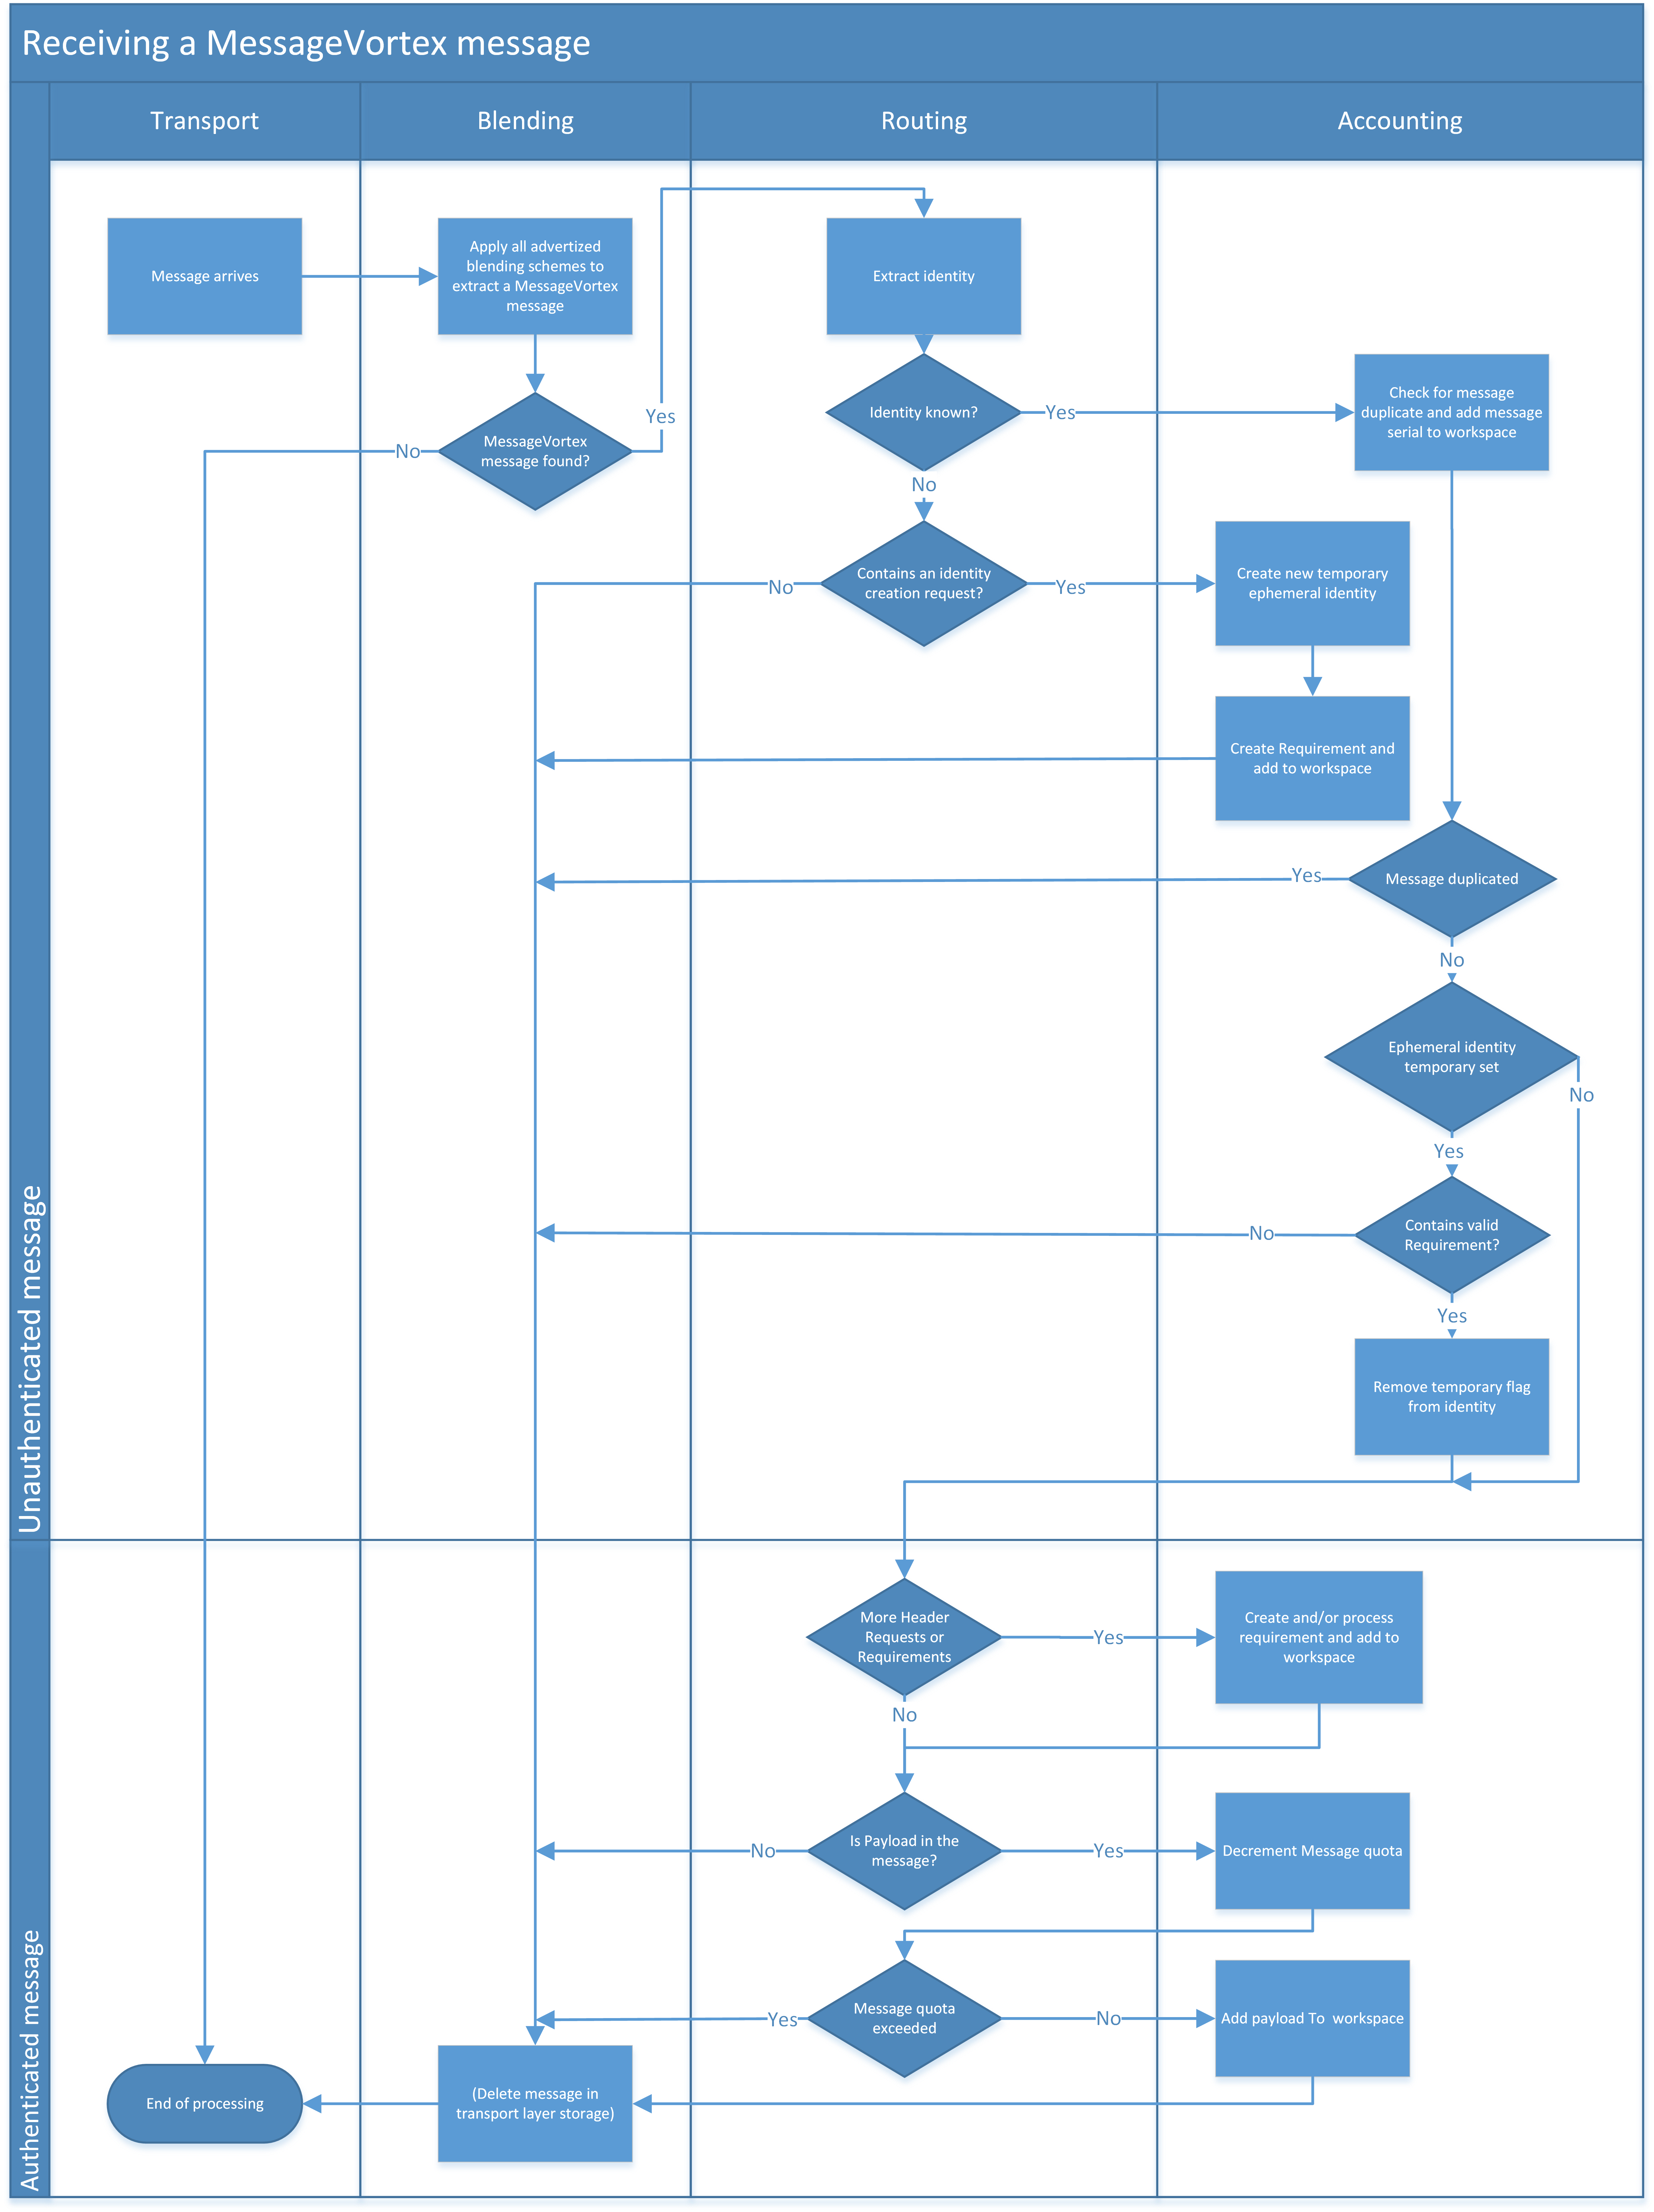
\includegraphics[height=0.75\textheight]{inc/flowchart_message_receiving}
	\caption{flow diagram showing processing of outgoing messages}
	\label{fig:msgReceiveProcessing}
\end{figure*}

As soon as the header requests are executed, the content is processed. The routing block operations are added to the workspace, and the mapping operations remain in the routing combo. 

\subsection{Processing of Outgoing Messages\label{sec:processingOutgoingMessages}}
In this section, we focus on the creation of new messages sent to the next-hop router. The message creation is triggered in a timed manner based on the content of the $RoutingCombo$ and then passed to the blending layer for blending.

A message sending is triggered by a routing block in the workspace, as shown in \cref{fig:msgSendProcessing}. The assembly instructions are processed to collect the payload blocks. Then the encryption is applied to the message and passed on to the blending layer for processing.

\begin{figure*}[ht]
	\centering
	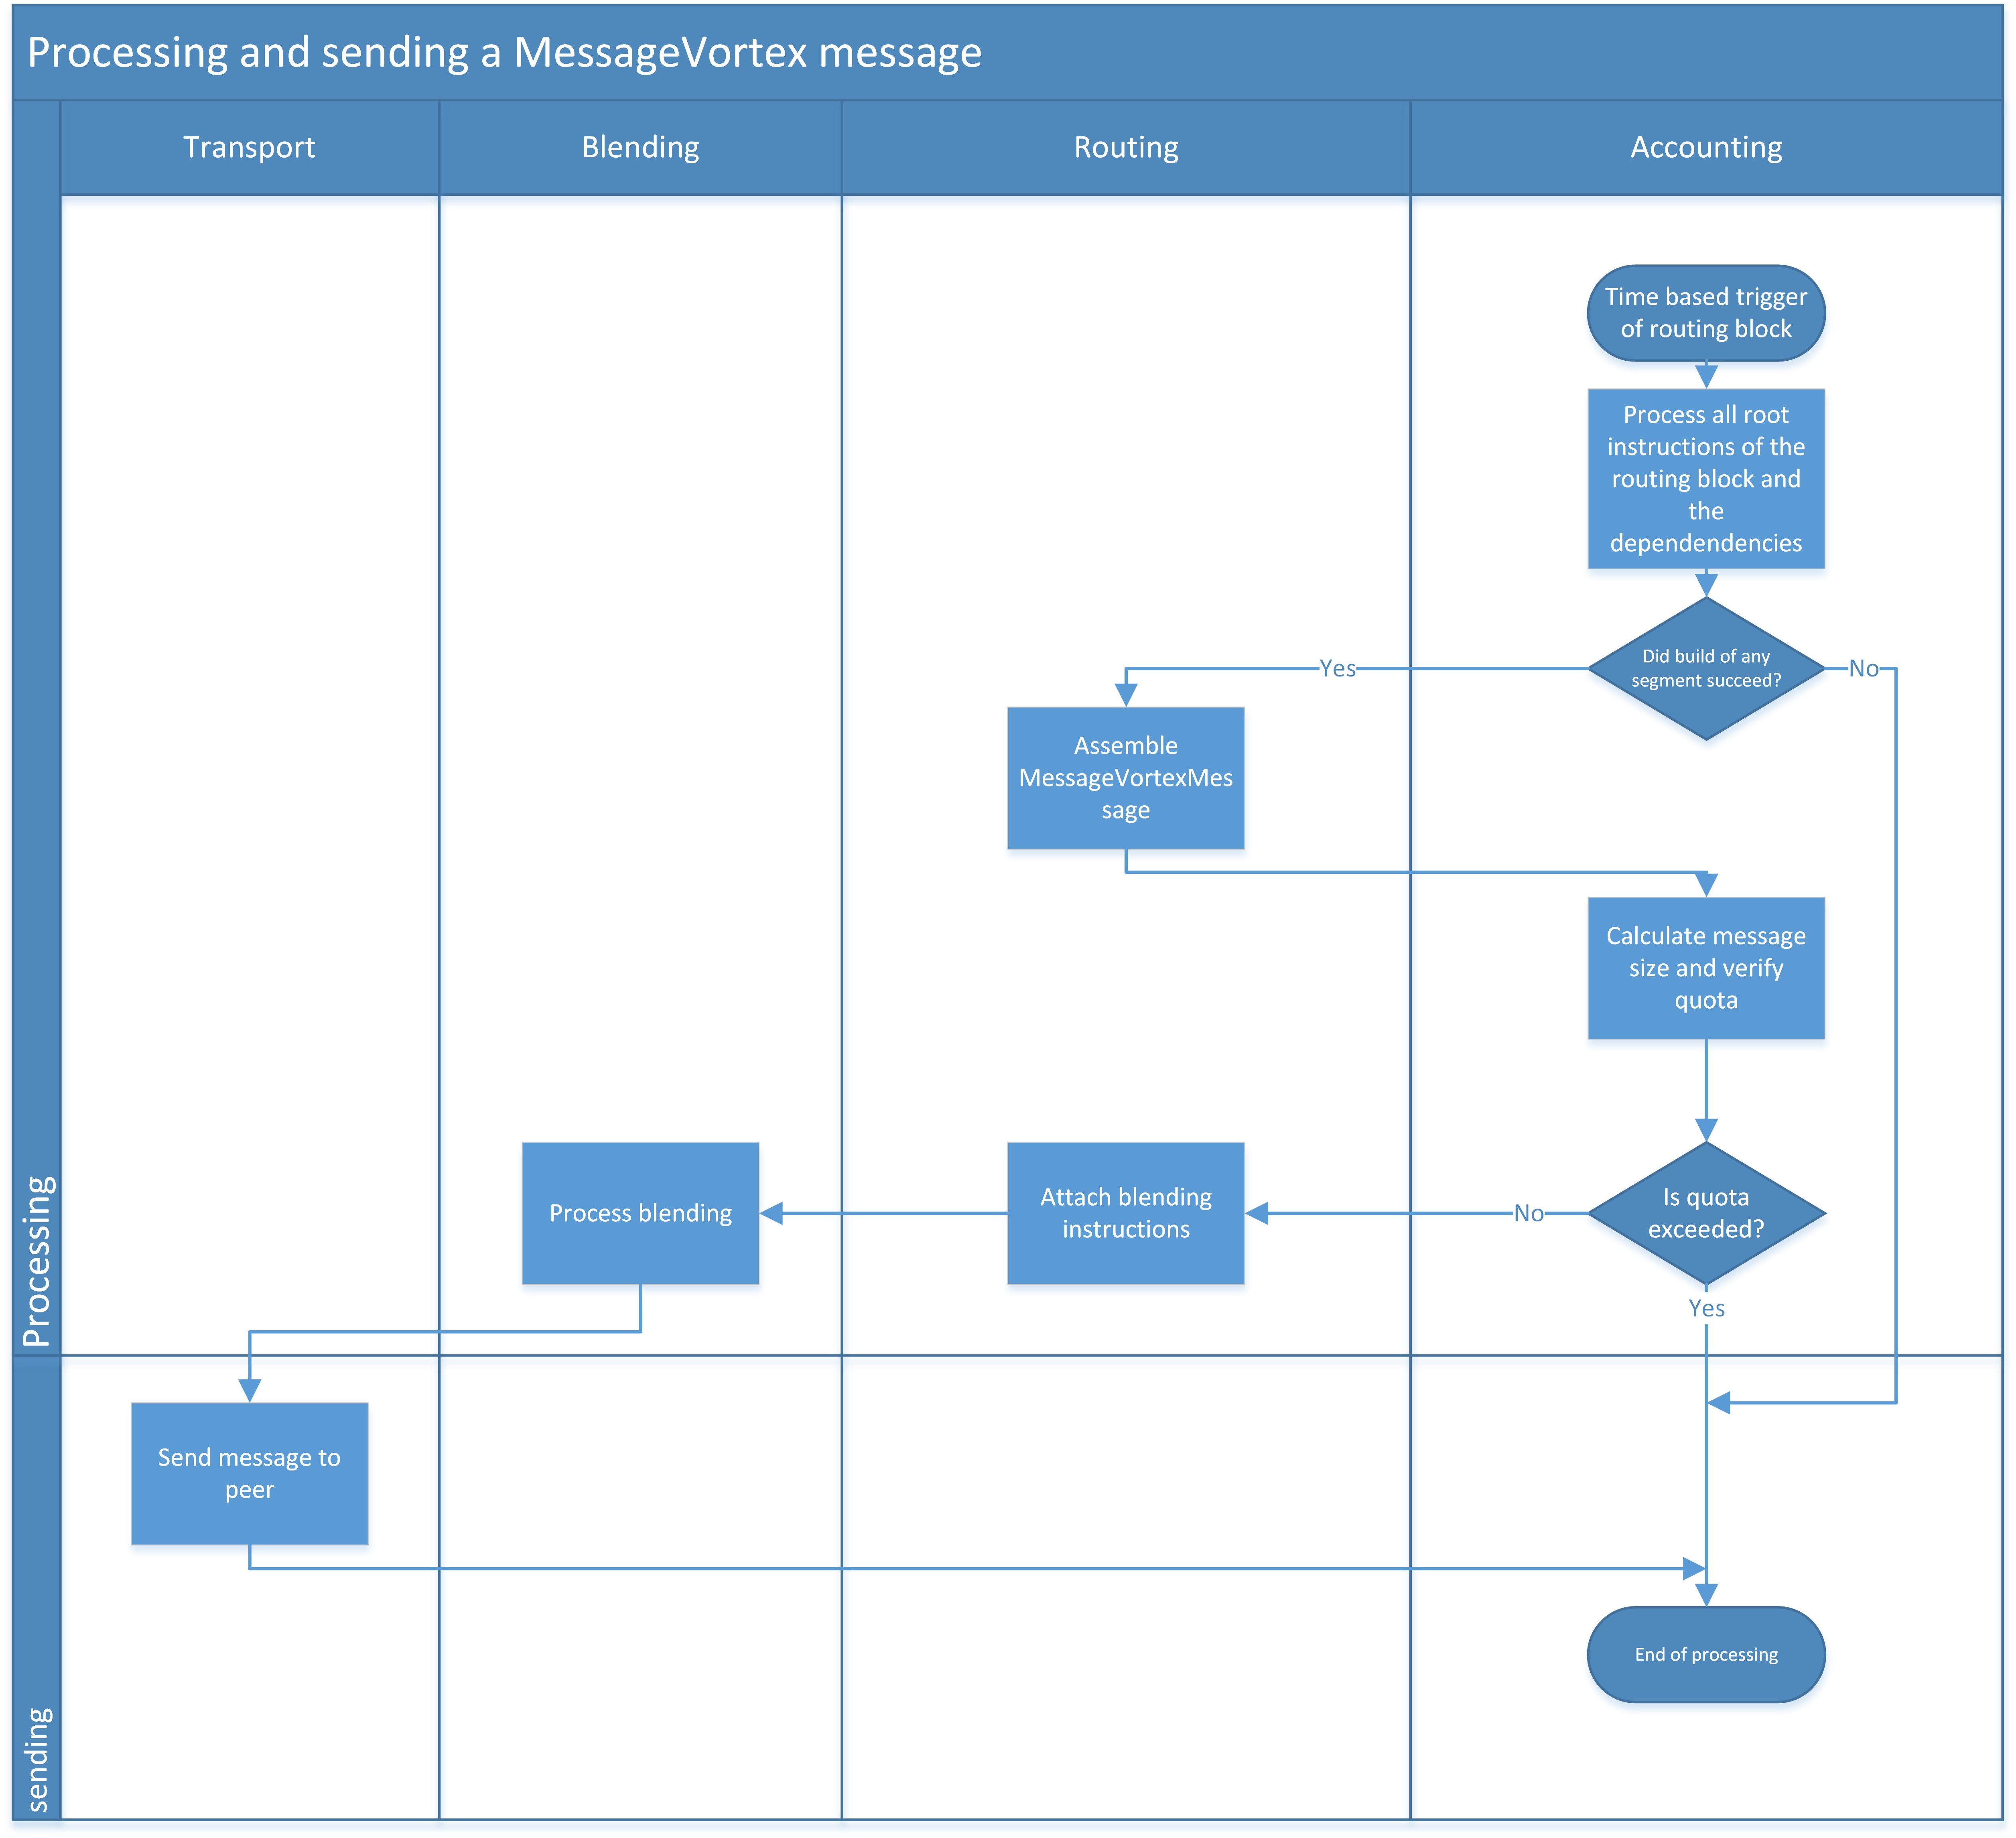
\includegraphics[width=0.90\textwidth]{inc/flowchart_message_sending}
	\caption{flow diagram showing processing of outgoing messages}
	\label{fig:msgSendProcessing}
\end{figure*}

All mapping operations are then carried out. If a payload has not yet been calculated, appropriate operations in the workspace are searched and executed to create the missing payloads. If a payload is not created successfully, the payload in the message is omitted. 

The message is assembled by building the $InnerMessageBlock$ with $cPrefix$, $header$, $routing$ from the routing combo and the payloads generated. This block is DER encoded and then encrypted with $peerKey$. The resulting octet-stream is prepended with $mPrefix$ from the routing combo and then passed to an appropriate blending layer for the requested transport using $blendingSpecc$.

The resulting message is a valid \VortexMessage, but the generating node has no relevant knowledge about the message or its content except for the recipient address.

\subsection{Implementation of Operations\label{sec:implOperations}}
In this section, we focus on the implemented operations. The operations outlined in \cref{sec:operations} were implemented in exactly the described manner. Additionally, we implemented a mapping operation, copying the content of one payload ID to another one. The implementation and its test showed some weaknesses related to the platform and implementation specifics, which are outlined further.

For our implementation, we used a HashMap to keep a list of all operations. The key of the HashMap is the output id of the resulting operations. Instead of proactively executing all operations to get all possible payload IDs, we build a dependency tree of all required prerequisites. A caching structure allows us to efficiently work with the results of all operations. If an operation expires, all cached output of the respective operations is invalidated. If a payload block expires or is overridden, all outputs taking input from this payload directly or indirectly are invalidated. This allows us to keep a very efficient and compact representation of the payload space, not wasting any memory without necessity.

The mapping operation became necessary when defining the system of specialized IDs as outlined in \cref{tab:workspaceId}. This usage of specialized workspace IDs makes the mapping of values from one  ID to another one a necessity. While theoretically doable in a two-step operation by applying an operation and its reverse, the mapping operation is far more efficient.

Some operations showed weaknesses. The splitPayload Operation was mathematically well designed. Due to differences in floating-point calculations (FP ops)when carried out on ARM and AMD based platforms, the result may differ when working with this operation. As an immediate result, we defined that all FP ops must be carried out as specified in \cite{IEEE754}. This allows us to have the same output of the splitting operation on all platforms and thus a constant result. Luckily in java, such behavior may be achieved by applying the \lstinline[columns=fixed,basicstyle={\normalsize}]{strictfp} keyword, which saved a lot of troubles and work.

Another problem that arose in practice was that applying a Gauloise field (GF) in the $addRedundancy$ and $removeRedundancy$ operations different to 8 or 16 make practical problems due to their resulting sizes. To simplify applying the transformation for the average computer working with 8 bits per byte only, we added a possibility for the node to signal which sizes of GFs are supported. This enables an implementation to focus on $GF(2^8)$ and $GF(2^{16})$ only.

A GF of size not equal to 8 or 16 requires the system to realign the data before processing, then applying the GF operations and converting it back to realign with 8-bit boundaries.

\section{Request handling}
In this section, we focus on handling requests and the replies to requests required by the protocol. As the replies are required but need to have the same properties as normal messages, we needed routing blocks for replies.

In general, any host may send a request to any other host. These requests normally involve the requirement for sender anonymity. The request itself is included in the \lstinline[columns=fixed,basicstyle=\normalsize]{HeaderBlock}. The reply block is provided in $requestReplyBlock$.

Requests are identified shown in \cref{fig:defRequest}. The tagging of the requests is necessary to identify the request provided.

\begin{lstfloat}[ht]
	\lstinputlisting[linerange={9-18},language=asn.1]{../../../../application-core-library/src/main/asn/MessageVortex-Requests.asn}
	\caption{Definition of a request}
	\label{fig:defRequest}
\end{lstfloat}

The routing blocks for replies must be different from normal routing blocks as they may otherwise be misused as ordinary sending blocks. A reply block for the request should always map to payload ID 32767, whereas a reply block for a normal user (to keep sender anonymity) should always map in workspace ID 0. That way, it is impossible to misuse reply blocks for normal messages.

A reply is sent as a special message block and must be mapped to workspace ID 128. A \VortexNode{} may accept a special block delivered to ID 0, but such behavior should never be assumed. Figure~\ref{fig:defReply} shows the definition of a reply. A reply is expressed in a special block. This special block contains a status of the request is either OK or a failure and may provide additional information such as the request's outcome.

\begin{lstfloat}[ht]
	\lstinputlisting[linerange={15-55},language=asn.1,multicols=2]{../../../../application-core-library/src/main/asn/MessageVortex-Replies.asn}
	\caption{Definition of a request}
	\label{fig:defReply}
\end{lstfloat}

\subsection{Requesting a new Ephemeral Identity\label{sec:newEID}}
One of the main requests for the protocol is the request for generating a new ephemeral identity. The goal of this operation is to create a non-hijackable workspace on a node while remaining anonymous. If having multiple \defref{eID}s on the same host, they must be unlinkable. Furthermore, it should be hard for an adversary to flood a \VortexNode{} with workspace requests to make a denial-of-service (DoS) attack.

\begin{lstfloat}[ht]
	\lstinputlisting[linerange={19-22},language=asn.1]{../../../../application-core-library/src/main/asn/MessageVortex-Requests.asn}
	\caption{Definition of an identity request}
	\label{fig:defCreateEID}
\end{lstfloat}

Requesting a new identity is easy. The only information required is the lifetime requested (see listing~\ref{fig:defCreateEID}). A \VortexNode{} may do any of the following operations:
\begin{itemize}
	\item Deny the request (even without an error message).
	\item Accept the request without a ``puzzle.''
	\item Accept the request under the condition a ``puzzle'' is solved.
\end{itemize}

Denial of a request does not necessarily lead to an error message. A \VortexNode{} sends only an error message if the node is a public node. All other nodes (stealth and hidden; see section{sec:vortexNodeTypes}) do not send an error message to not leak their existence.

If a request is accepted, the \VortexNode{} replies either with an ``ok'' or a ``puzzle required'' status.

\begin{lstfloat}[ht]
	\lstinputlisting[linerange={9-34},language=asn.1,multicols=2]{../../../../application-core-library/src/main/asn/MessageVortex-Requirements.asn}
	\caption{Definition of a requirement}
	\label{fig:defRequirements}
\end{lstfloat}

As currently supported puzzles, two possible answers are foreseen by the protocol:
\begin{itemize}
	\item Solving a CPU bound hash puzzle 
	\item Paying a fee in a digital currency
\end{itemize}

The CPU bound puzzle is a hash-based puzzle. The \VortexNode{} provides a bit string for the identity. The header has to be resent so that the requested hash of the DER-encoded header starts with the bit sequence provided. there are two ways of keeping track of these puzzles:

\begin{itemize}
	\item Generate puzzles in a reproducible way\\
	This is the more elegant way of puzzles. Instead of keeping track of the puzzles, we generate the hash by applying the following function $left(MAC(K^1_{identity} | <\text{host secret}> | <\text{ date and hour }>),\text{hourly complexity in bits})$. This method has some ups and downs. On the positive side, we do not need to keep track of all puzzles provided to identities. Instead, we just check if a puzzle provided matches an appropriate challenge of the last hours. This host cannot be flooded with identity creation requests as it does not need to keep track of the requests. Instead, it must keep a list of successful serials that requested a quota increase as there it would be possible to replay the request to increase the quotas. This is not comparable to the costs for an attacker as we have only to keep a list of integers where the PoW has been solved.
	\item Store random puzzles during their validity time\\
	This method is straight forward. It requires an entry in a table per puzzle and only for the lifetime considered. 
\end{itemize}

The second approach has a huge downside: A DoS attack is feasible. Given the fact that we need to store the key (1KB max), the date and time of expiry 4 bytes (epoch), and the bit sequence (up to 8 bytes). This means that we require millions of requests to flood a host. Since the keys do not need to be strong (an adversary does not intend to use them; It is just a DoS attack), this attack is doable with considerable effort. This is why we favor the first approach.

\subsection{Replacing an Existing Node Specification or Proving a Sender Identity\label{sec:replaceID}}
As users tend to change transport layer addresses, keys might become insecure, or transport services are no longer available, we need means of upgrading keys or replacing them with newer transport addresses. This may be done with a $HeaderRequestReplaceIdentity$ request as shown in \cref{fig:reqReplaceIdentity}. This request allows in a cryptographically secured way to exchange keys and transport endpoints by the respective owners.

\begin{lstfloat}[ht]
	\lstinputlisting[linerange={23-30},language=asn.1]{../../../../application-core-library/src/main/asn/MessageVortex-Requests.asn}
	\caption{Definition of an identity replace request}
	\label{fig:reqReplaceIdentity}
\end{lstfloat}

By signing the request, the sender proves that he is in possession of the old key. By omitting the new node specification, a user may bind an existing \defref{eID} to a real-world identity. This is useful for securing endpoint identities if required. However, such a secured identity should only be used for endpoint messages and not for routing, as this would shorten the secured path of the message.

A \VortexNode{} may reply with a ``quotaStatus'' message if the node owner decides to assign a different (possibly unlimited) quota to the identity. 

\subsection{Replacing an Existing Reply Block\label{sec:replaceMURB}}
For sender anonymity, a sender may provide a reply block for single or multiple uses (SURBS and MURBS). These routing blocks use \defref{eID}s, which have by definition a limited lifespan. In this section, we focus on the implementation details for requests replacing such reply blocks.

A routing block has a limited lifespan, which is directly limited by the \defref{eID}s involved. The first expiring \defref{eID} invalidates the block unless redundant paths are included. In this case, only redundancy would be reduced. To keep a message intact, even if a reply block of an anonymous sender expires, the sender may replace any existing reply block with a new routing block.

In the case an owner wants to replace an existing routing block with a new one, it is sufficient to send an empty message to the respective \defref{eID}. Within the routing block, the sender provides one or more new $replyBlock$ replacing all old existing ones. As the header is signed by the private key of the \defref{eID}s owner, this operation is safe.

\chapter{Accounting Layer Implementation}\label{sec:accountingImplementation}
The accounting layer is keeping track of all operations allowed to a message. In this section, we list the tasks fulfilled by the accounting layer and make a precise outline of them.

The accounting layer Keeps a list of the following information:
% List duplicated in Accounting layer in implementation and protocol
\begin{itemize}
	\item $\mathbf{eID[]}\langle expiry, pubKey, mesgsLeft, bytesLeft \rangle$\\
	\item $\mathbf{Puzz[]}\langle expiry, requestHeader, puzzle \rangle$\\
	or\\
	$\mathbf{Puzz[]}\langle dateAndHour, puzzleSizeNewIdentity, basePuzzleSizeQuta \rangle$\\
	\item $\mathbf{Replay[]}\langle expiry, serial, numberOfRemainingUsages \rangle$\\
\end{itemize}

The list of all \defref{eID}s is kept in the accounting layer together with their quotas and expiry. The accounting layer triggers the deletion of the workspace assigned to it upon its expiry. Each \defref{eID} has assigned two quotas. The $messageQuota$ limits the number of messages containing payload blocks to be routed. This quota is measured upon the arrival of a message (inbound only). The $bytesLeft$ quota is a sizing quota and is measured outbound. This quota is applied to all outbound messages regardless of their content.

The $puzz[]$ list with $requestHeaders$ is only required if relying on random user puzzles. This would lead to an implementation that is simple but may be flooded with \defref{eID} requests. The second list requires only an entry per hour. The number of entries is limited by the number of hours a puzzle is accepted. The puzzle is built by calculating  $MAC\left(K^1_{eID} | globalSecret | dateAndHour ), puzzleSizeNewIdentity\right)$. That way, a DoS attack by flooding the puzzle table is no longer feasible.

The last list is the list for replay protection $Replay[]$. This list is a list of serials, and their remaining usages is an effective replay protection. A serial is only allowed to be processed if the serial has not reached the maximum number of replays. As a header block typically has only a limited lifespan, this is a very short list. Flooding is not very effective as a host may limit the number of entries in this list. The only identity suffering from that measure would be the identity assigned to the serial as serials from this \defref{eID} would suffer incomplete replay protection and thus endanger its quotas.

In \cref{tab:protoReplyCrit}, we show under what circumstances a reply to a header request should be sent. The capitalized words MAY, MUST, SHOULD, and SHOULD NOT are used as defined in RFC2119\cite{rfc2119}. 
\begin{table*}[ht]
	\centering\scriptsize
	\begin{tabular}{|l|l|l|l|l|}\hline
		\diaghead{\theadfont Request Criteria}{Request}{Criteria} & \thead{\begin{minipage}{2.5cm}unknown identity\\cleartext\end{minipage}} & \thead{\begin{minipage}{2.5cm}unknown identity\\ encrypted\end{minipage}} & \thead{\begin{minipage}{2.5cm}expired identity\\encrypted\end{minipage}} & \thead{\begin{minipage}{2.5cm}known identity\\encrypted\end{minipage}}\\\hline
		newIdentity         & SHOULD NOT    & MAY         & Invalid (Error)     & Invalid (Error)\\              
		queryPeer           & MUST NOT      & MUST NOT    & MAY                 & MAY\\        
		queryCapability     & SHOULD NOT    & MAY         & MAY                 & MUST \\
		messageQuota        & MUST NOT      & MUST NOT    & MAY                 & MUST \\              
		transferQuota       & MUST NOT      & MUST NOT    & MAY                 & MUST \\\hline             
	\end{tabular}    
	\caption{Requests and the applicable criteria for replies}
	\label{tab:protoReplyCrit}
\end{table*}

\chapter{Usability Related Implementation Details}\label{sec:usabilityImplementation}
Usability is one of the foremost criteria for user acceptance. As we have no chance to create a nice User interface competing with existing ones, we went for a different approach. We use our \VortexNode{} as an IMAP/SMTP proxy. That way, we can send with any email client \VortexMessages. To do so, we had to introduce an addressing scheme compatible with email and the support of their clients but not creating any collisions with the existing email address schemes.

These schemes are discussed in the next section. After that, we address the problem of linking to user agents and transparency issues.

\section{Addressing and address representations}
An endpoint always requires a public key and a transport endpoint. As we have no central infrastructure, we need a defined way to exchange addresses. These addresses need to be uniquely identifiable and have to work with clients. In this section, we focus, therefore, on the implementation details of such an address.

If we want to use common email or XMPP clients, we must support an address format compatible with the client but produces no collisions with ordinary addresses. Luckily experiments showed that clients are not very restrictive in the acceptance of addresses. Most clients required either an at sign between two letters or, additionally, at least a dot in the domain part of the address. \cite{rfc5321} and \cite{rfc5322} specify the format for email addresses and \cite{rfc6120} does the same for XMPP. For both formats, a double dot (``..'') in the local part is illegal. Clients do not seem to catch this exception. We, therefore, defined our addresses as follows.


For email:
\begin{lstlisting}[language=EBNF]
	localPart         = <local part of address>
	domain            = <domain part of address>
	email             = localPart "@" domain
	keySpec           = <BASE64 encoded AsymmetricKey [DER encoded]>
	smtpAlternateSpec = localPart ".." keySpec ".." domain "@localhost"
	smtpUrl           = "vortexsmtp://" smtpAlternateSpec]
\end{lstlisting}

For XMPP:
\begin{lstlisting}[language=EBNF]
	localPart         = <local part of address>
	domain            = <domain part of address>
	resourcePart      = <resource part of the address>
	jid               = localPart "@" domain [ "/" resourcePart ]
	keySpec           = <BASE64 encoded AsymmetricKey [DER encoded]>;
	jidAlternateSpec  = localPart ".." keySpec ".." 
	domain "@localhost" [ "/" resourcePart ]
	jidUrl            = "vortexxmpp://" jidAlternateSpec]
\end{lstlisting}

This allows using of a regular client to host an \VortexMessage{} endpoint address. To avoid unintentional routing of an address to through a non-\VortexNode{}, we defined ``localhost'' as the general domain part. The local part in the email is restricted to 64 bytes, whereas XMPP specifies 1024 bytes as the local part's size limit. Our experiments showed, however, that none of the clients enforce these limits.

The respective URLs are defined in the standard to provide a unified mean for URLs to be properly identified by a system. This allows a unified usage of mechanisms such as QR codes across all platforms.

\section{Linking to Common User Agents}
From an academic perspective, the protocol linking as a proxy is easy. Real-world implementation showed, however, many caveats. We will focus on these problems in this section and note workarounds where possible.

When combining data on asynchronous message protocols, we always have two possibilities. Either work as a transparent proxy for a single view or combine multiple sources. Another option is always creating a local repository with the downside that such a repository may not be shared with other devices.

For all protocols, we have to mention that using the \VortexNode{} as a transparent proxy is not always doable for two reasons. First, we must do a man in the middle (MITM) attack when proxying outbound or inbound connection. If such connections are encrypted, this is a problem due to the breach of the trust chain involved. Solving this in an enterprise environment is easy, as we can control the trust store. Working with mobile operating systems such as android or iOS, access to trust stores are complex and, under some circumstances, even prohibited.

Another problem is that such MITM attacks are easily detected when employing DANE (\cite{rfc6698,rfc7672}) or similar technologies. Within all protocols, analyzed certificate-based authentication is very uncommon. But such authentication would break if we do a MITM.

When sending an email, we can use authenticated SMTP on the client submission ports. This may be realized either as a transparent proxy or as a store and forward solution with very few downsides. When working as store and forward, we have the downside that in case of networking failure, the node may delay or lose (in a worst-case scenario) the message without the user knowing it as the client successfully sent the message. We developed an easy workaround for this scenario: Our SMTP implementation binds on 127.0.0.1 only and accepts a dummy password. Simultaneously, we build a second connection to the provider's SMTP channel and authenticate. As soon as the envelope is complete, we decide whether the recipient is a \VortexNode{} (easily identifiable by the address).  If not, we send the envelope to the providers SMTP connection and strictly forward from there on all traffic between the two. If the recipient is a \VortexNode{}, we use a pseudo blending layer that packs an appropriate routing block and the plain text message as a single payload into a pseudo \VortexMessage{} and deliver this message to the routing layer. The routing layer then, unaware of the message's pseudo nature, handles the message. It does the first encryption operation and applies then the operations to send the message to all next hops with the appropriate routing blocks.

When receiving messages by mail, things get quickly more complex. For our experiments, we used POP3 as a protocol. This protocol is somewhat similar to SMTP and allows normal store and forward operation. This means that we may fetch mail from a central infrastructure. This fetching is triggered by the fetching of the client, which is thus almost delay-less. As with POP3 mails are stored locally, we have no problems as the client fetches and stores the mail. Considering IMAPv4, we have a couple of very relevant differences. Unlike POP3, IMAPv4 stores and organizes messages on the server. The main advantage is that due to the central storage, multiple devices may access the messages simultaneously. Since all clients use the same storage, a unified view is possible. Unfortunately, all attempts generating a globally unique id for messages failed so far, and client support for such a feature is sparse. In an ideal world, we would have a unified view out of one or more \MessageVortex{} transport layer accounts and our regular mail, whereas the \VortexMessages{} are stored in the respective transport layer account and dynamically merged into the regular email store. 

Such a store would have huge benefits compared to the current solution. It would allow unified storage and offering simultaneous access for multiple devices. The problems to be solved are numerous. We need unified storage for configurations including \defref{eID}s and workspaces. Furthermore, we need a lock to avoid concurrency issues with simultaneously running \VortexNodes{}. The unified view requires intelligence so that it is able to keep all \VortexMessages{} on the transport layer account, whereas ordinary emails are kept on the respective account. The housekeeping of the transport layer account needs to be done in a credible way. 

\chapter{Efficiency Related Implementation Details}\label{sec:efficiencyImplementation}
In the following section, we focus on the storage management of \VortexNodes{}. As they do run on mobile and similar devices, low resource consumption is essential for our system. We mainly focus on memory and CPU consumptions. Network bandwidth overhead and their related problems are discussed in \cref{sec:analysis}.

\section{Node Storage Management}
In most mobile devices, storage is very limited. This applies to the disk storage but is exceptionally true for the RAM of such devices. Our protocol supports the minimization of storage footprints in two ways.
\begin{enumerate}
	\item Every node may minimize the storage footprint by signaling that only a small footprint is possible through the capability block.
	\item Every node may minimize the number of \defref{eID}s accepted.
\end{enumerate}

The runtime portion of RAM required may be minimized as the concurrently needed RAM is limited to the event-triggered Routing blocks, respectively their trigger blocks. Listing~\ref{lst:defUsage} defines two type of windows. The absolute time (\texttt{AbsoluteUsagePeriod}) denominates the time interval the item is valid in an absolute UTC-based manner. The relative timing (\texttt{RelativeUsagePeriod}) furthermore limits the validity window measured relative to the time of arrival. The real validity time is formed as the intersection out of the two timings, whereas both may be omitted by definitions.

\begin{lstfloat}[ht]
	\lstinputlisting[linerange={10-23},language=asn.1]{../../../../application-core-library/src/main/asn/MessageVortex-Helpers.asn}
	\caption{Definition of a timing trigger}
	\label{lst:defUsage}
\end{lstfloat}

The \texttt{ReplyCapability} as shown in listing~\ref{lst:defCapabilityReply} allows a \VortexNode{} to effectively limit the memory usage. 
\begin{lstfloat}[ht]
	\lstinputlisting[linerange={61-91},language=asn.1]{../../../../application-core-library/src/main/asn/MessageVortex-Replies.asn}
	\caption{Definition of a capability reply block}
	\label{lst:defCapabilityReply}
\end{lstfloat}


\subsection{Storage Management of Ephemeral Identities,  Operations, and Payload Blocks}
The ephemeral identity (\defref{eID}) is the overarching unit of users data. In a normal message server, it may be comparable with the storage required for the queues. Unlike a message queue, \VortexMessages{} are not only kept until sent. \VortexMessages{} have different properties as we have a timed store-and-forward behavior. As a general rule, no data lives longer than its \defref{eID}.

When an \defref{eID} is requested an absolute \texttt{UsagePeriod} (a timezone bound time) is specifies with an \texttt{AbsoluteUsagePeriod} is specified (see \cref{lst:defUsage}). Unless used for reply blocks (MURBs), \defref{eID} have a very limited lifespan of a couple hours. This minimizes any storage footprint associated with an \defref{eID}. 

\begin{lstfloat}[ht]
	\lstinputlisting[linerange={85-114},language=asn.1,multicols=2,basicstyle=\tiny]{../../../../application-core-library/src/main/asn/MessageVortex-Schema.asn}
	\caption{Definition of a header block}
	\label{lst:defHeaderBlock}
\end{lstfloat}

Every header block contains a relative and possibly an absolute \texttt{UsagePeriod}. A receiving node calculates a headers' lifespan by intersecting an absolute lifespan and a relative lifespan. All elements of a \VortexMessage{} inherit this lifespan. Therefore, payload blocks and operations, as well as the routing blocks expire simultaneously within a workspace.

Furthermore, A node signals additional boundaries in the CapabilityReplyBlock (see \cref{lst:defCapabilityReply}). with this block, a \VortexNode{} may limit the storage required even further. By specifying low boundaries for the maximum simultaneously usable payload blocks in a workspace and their maximum size, we can effectively limit the size of the payload data of a single workspace. The number of simultaneously active operations is similarly limited by specifying \texttt{maxBuildOps}.

\subsection{Life-cycle of Requests}
Requests have a separate lifecycle. As a Request may exist prior to a corresponding workspace, which is typically assigned to a proof of work, such requests may be subject to DoS attacks by flooding the memory of a node. All requests immediately executed have no direct memory requirements. However, requests containing a PoW cycle require to maintain the state. 

While this is considered a minor issue as it is very likely that nodes will first collapse due to their network load, we can still address this issue by using a secret generator instead of a list based as outlined in \cref{sec:newEID}. By using such a generator, we minimize the impact of a very sudden increase in requests while keeping the local memory requirements to an absolute minimum. 

%\section{Overhead Minimization in Message}
%\fxwarning{complete section}

\subsection{Minimizing the Memory Footprint of Message Processing}
To limit the memory footprint of message processing, we reduced the information relevant to be kept in memory by structuring the message accordingly. A node may first extract the first header block, which is equivalent to the block size of the cipher used to encrypt the header block. If the message is invalid due to a non-existent message, we may stop there. We then start decoding the header prefix block, and if successful, the header, which is typically less than 1KB in size unless it contains a routing block. Each routing block is $~1 \frac{KB}{hop}$ in size (assuming a 2048 bit asymmetric key). Only the first couple of bytes have to be read, and the vast majority may then be streamed as it is mainly a binary, encrypted blob containing subsequent hops. All subsequent blocks (routing and payload blocks) are not required to be kept in memory simultaneously. Instead, we may stream them into a data structure on persistent storage. Operations on the payload block are suitable for streaming processing either. For $encryption$ and $split/merge$ operations this is obvious. the transformation and retransformation of the $redundancy$ operations may be done with a lookup table. It requires, however, 256 KB on disk for a $GF(2^{16})$ transformation. The matrix operations are comparably small again as they may be carried out on an element per element base with simple, calculable lookups. 

We may therefore conclude that while a workspace may require considerable storage for storing all payload and routing blocks, the processing of a message can be done in a very memory efficient manner if required. We may execute all calculations on payload blocks in a streamed manner, and all blocks required for routing are either very small or may be streamed again.




